\documentclass[a4paper, 10pt]{article}%тип документа

%отступы
\usepackage[left=2cm,right=2cm,top=2cm,bottom=3cm,bindingoffset=0cm]{geometry}
\usepackage{amssymb}
%Русский язык
\usepackage[T2A]{fontenc} %кодировка
\usepackage[utf8]{inputenc} %кодировка исходного кода
\usepackage[english,russian]{babel} %локализация и переносы

%Вставка картинок
\usepackage{graphicx}
\graphicspath{{pictures/}}
\DeclareGraphicsExtensions{.pdf,.png,.jpg}

%Графики
\usepackage{pgfplots}
\pgfplotsset{compat=1.9}

%Математика
\usepackage{amsmath, amsfonts, amssymb, amsthm, mathtools}
\begin{document}

\date{}
\author{}
\title{Вопрос по выбору:\\
Маятник Фуко, геофизическое проявление силы Кориолиса, определение угловой скорости вращения Земли}
\maketitle
\large
\section*{Введение}
Маятник Фуко представляет собой массивный шар, подвешенный на длинной нити и совершающий малые колебания около положения равновесия. Если бы Земля была ИСО, то в случае выведения маятника из положения равновесия и предоставления его воздействию только силам тяжести и натяжения нити он бы совершал колебания только в одной вертикальной плоскости. Однако в действительности плоскость колебаний совершает вращение вокруг вертикальной оси, что доказывает влияние неинерциальной силы Кориолиса, возникающей в результате вращения Земли вокруг своей оси, на движения маятника и подтверждает факт того, что наша планета является НеИСО.


На тело, рассматриваемое относительно НеИСО, кроме внешних сил могут действовать силы инерции. Допустим, в некоторой НеИСО на материальную точку массой m действует некоторая сила $\vec{F}$ и равнодействующая сил инерции $\vec{F}_{\text{ин}}$. Можно записать второй закон Ньютона:
\[ m\vec{a} = \vec{F} + \vec{F}_{\text{ин}}, \quad \text{где} \quad \vec{F}_{\text{ин}} = \vec{F}_{\text{пост}} + \vec{F}_{\text{ц.б.}} + \vec{F}_{\text{кор}}  \]
\[ \vec{F}_{\text{пост}} =  - m\frac{d\vec{V}_{0}}{dt}, \quad \vec{F}_{\text{ц.б.}} = -m\vec{\omega}\times \left({\vec{\omega}\times\vec{r}}\right) - m\frac{d\vec{\omega}}{dt}\times\vec{r}, \quad \vec{F}_{\text{кор}} = -2m\vec{\omega}\times\vec{v}\]
В случае с маятником буду рассматривать только кориолисову силу $\vec{F}_{\text{кор}}$, зависящую от массы груза $m$, скорости его движения $\vec{v}$ и угловой скорости вращения Земли $\vec{\omega}$, поскольку именно она перпендикулярна к плоскости качаний маятника и существенно влияет на её вращение.

\section*{Маятник с точки зрения ИСО}
Предположим, что маятник находится на некоторой широте $\varphi$ (рис. 1). В таком случае вектор угловой скорости Земли $\vec{\omega}$ можно разложить на вертикальную и горизонтальную составляющие: $\vec{\omega} = \vec{\omega}_{\text{в}} + \vec{\omega}_{\text{г}}$.
Слагаемое $\omega_{\text{г}}$ влияет на силу натяжения нити, а $\omega_{\text{в}}$ - на рассматриваемое вращение плоскости колебаний маятника. Тогда 
\[ \omega_{\text{в}} = \omega\sin \varphi = \frac{2\pi\sin \varphi}{T_{\text{З}}}, \quad T_{\text{М}} = \frac{2\pi}{\omega_{\text{в}}} = \frac{T_{\text{З}}}{\sin \varphi}, \quad \omega = \frac{2\pi}{T_{\text{М}}\sin \varphi}\]
Таким образом, зная широту расположения маятника и его период совершения полного оборота его плоскости колебаний, можно найти угловую скорость вращения Земли.

\newpage
\section*{Маятник с точки зрения НеИСО}
Аналогично первому варианту, для маятника, расположенного на широте $\varphi$, разложим $\vec{\omega}$ на $\vec{\omega}_{\text{в}}$ и $\vec{\omega}_{\text{г}}$. В данном случае дополнительно разложим $\vec{\omega}_{\text{г}}$ на $\vec{\omega}_{\text{$\bot$}}$ и $\vec{\omega}_{\text{$\parallel $}}$ так, что $\vec{\omega}_{\text{$\bot$}}$ перпендикулярна плоскости колебаний в данный момент, а $\vec{\omega}_{\text{$\parallel $}}$ лежит в ней (рис. 2).
В таком случае можно записать второй закон Ньютона с учётом сил Кориолиса:
\[ m\vec{a} = m\vec{g} - 2m\vec{\omega}_{\text{в}}\times\vec{v} -2m\vec{\omega}_{\text{$\bot$}}\times\vec{v} - 2m\vec{\omega}_{\text{$\parallel $}}\times\vec{v}  \]
Сила $-2m\vec{\omega}_{\text{в}}\times\vec{v}$ является интересующей нас составляющей, так как она перпендикулярна плоскости колебаний и вызывает её вращения. Сила $-2m\vec{\omega}_{\text{$\bot$}}\times\vec{v}$ действует вдоль нити маятника, из-за чего её длина и, соответственно, период колебаний маятника могут незначительно меняться, что можно не учитывать в приблизительных расчётах.
Силой $- 2m\vec{\omega}_{\text{$\parallel $}}\times\vec{v}$, перпендикулярной плоскости колебаний тоже можно пренебречь, так как, во-первых, при малом угле отклонения $\alpha$ она мала, а во-вторых, при смене направления скорости груза она тоже меняет направление и компенсирует своё прежнее воздействие.
Таким образом, уравнение движения маятника в НеИСО имеет следующий вид:
\[m\frac{d^2\vec{r}}{dt^2} = -\frac{mg\vec{r}}{r} - 2m\vec{\omega}_{\text{в}}\times\frac{d\vec{r}}{dt}  \]
Вектор $\vec{r}$ можно разложить по горизонтальным осям X и Y, тогда оно будет сводиться к следующим уравнениям, описывающим проекцию груза на горизонтальную плоскость:
\[\frac{d^2x}{dt^2} + \omega_0^2x=2m{\omega}_{\text{в}}\frac{dy}{dt},  \qquad \frac{d^2y}{dt^2} + \omega_0^2y=-2m{\omega}_{\text{в}}\frac{dx}{dt}\]
Здесь была введена собственная частота колебаний маятника $\omega_0 = \sqrt{\frac{g}{r}}$. К решению данной системы можно прийти, введя комплексную функцию $z=x+iy$. Тогда, домножив первое уравнение на $i$ и сложив его со вторым, получим уравнение для введённой функции:
\[\frac{d^2z}{dt^2} + 2i{\omega}_{\text{в}}\frac{dz}{dt}+\omega_0^2z=0  \]
Далее положим $z=z_0e^{i\Omega t}$. Подставив, получим
\[-\Omega^2-2{\omega}_{\text{в}}\Omega+\omega_0^2=0, \quad \text{тогда} \quad \Omega=-{\omega}_{\text{в}}\pm\sqrt{{\omega}_{\text{в}}^2+\omega_0^2}\]
Таким образом, получаем общее решение уравнения для $z$:
\[z=z_{01}e^{-i{\omega}_{\text{в}}t-i\omega_1t}+z_{02}e^{-i{\omega}_{\text{в}}t+i\omega_1t}, \quad \text{где} \quad \omega_1=\sqrt{{\omega}_{\text{в}}^2+\omega_0^2}\]
Затем, положив $z_{01}=a_1e^{i\varphi_1}, \quad z_{02}=a_2e^{i\varphi_2}$ и отделив действительную ($x=\text{Re}\,z$) и мнимую ($y=\text{Im}\,z$) части, получим искомое решение:

\[x =  a_1 \cos [(\omega_1 + \omega_{\text{в}})t - \varphi_1] + a_2\cos [(\omega_1-\omega_{\text{в}})t + \varphi_2]  \]
\[y = -a_1 \sin [(\omega_1 + \omega_{\text{в}})t - \varphi_1] + a_2\sin [(\omega_1-\omega_{\text{в}})t + \varphi_2]  \]
Данная система уравнений содержит четыре произвольние постоянные $a_1, a_2, \varphi_1, \varphi_2$, определяемые начальными условиями.

В рассматриваемой ситуации $\omega_{\text{в}} \ll \omega_0 \approx \omega_1$, поэтому полученные соотношения описывают обычные колебания математического маятника с периодом $T \approx \frac{2\pi}{\omega_0} = 2\pi\sqrt{\frac{r}{g}}$, причём плоскость, в которой они совершаются, медленно поворачивается, что опять же подтверждает вращение Земли.

\begin{figure}[h]
    \center{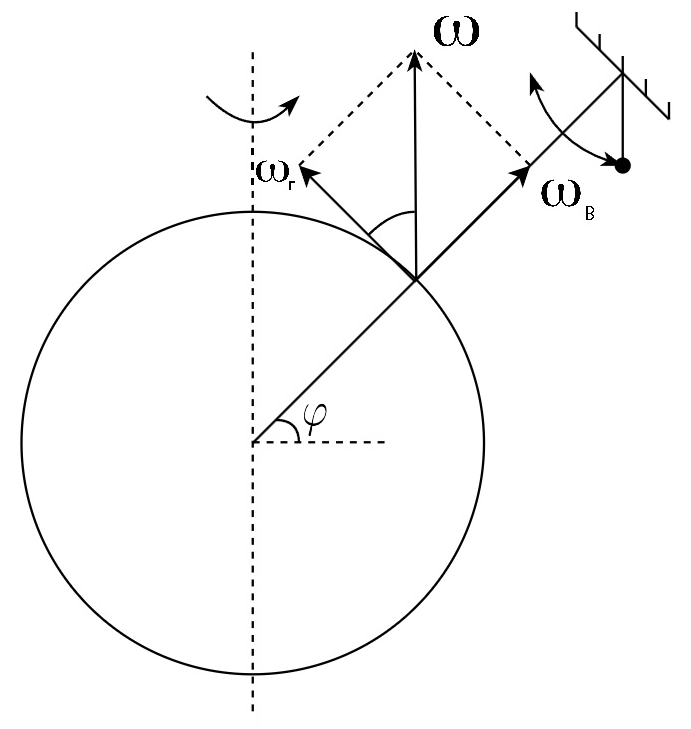
\includegraphics[scale=0.4]{схема.png}}
    \caption{ИСО}

\end{figure}

\begin{figure}[h]
    \center{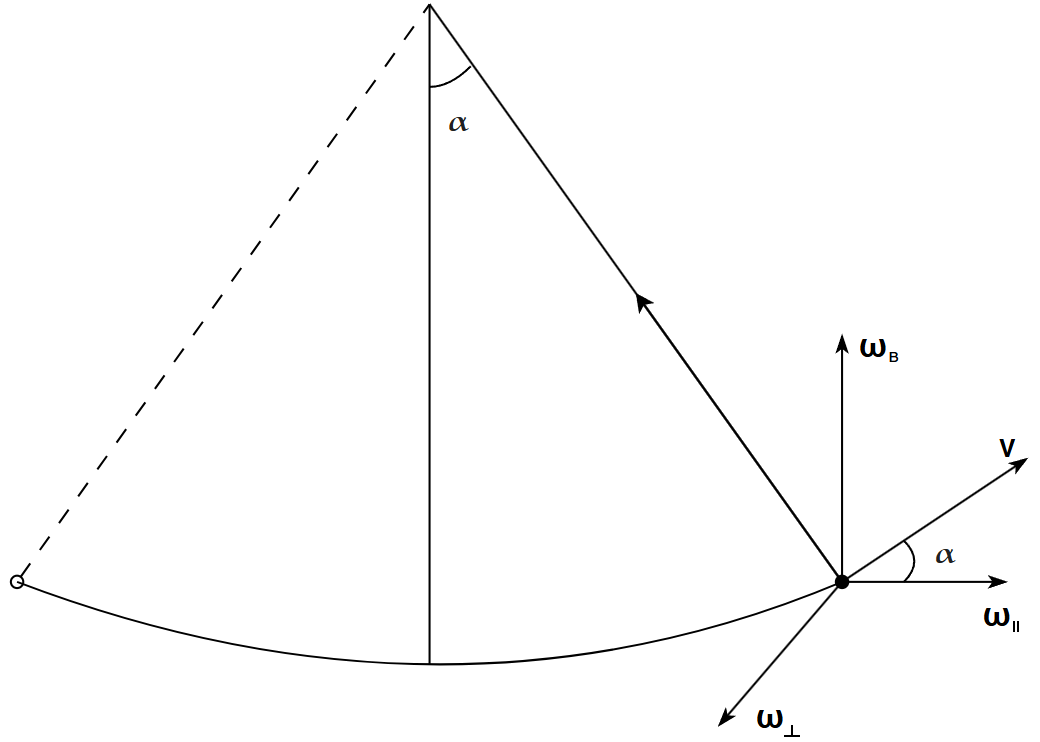
\includegraphics[scale=0.4]{схема 2.png}}
    \caption{НеИСО}

\end{figure}

\begin{figure}[h]
    \center{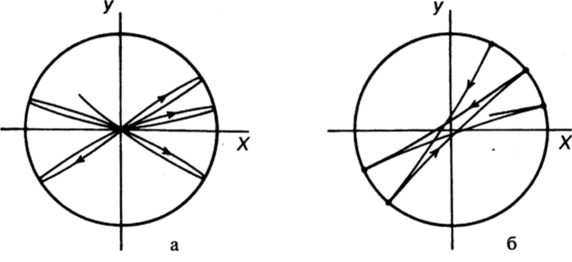
\includegraphics[scale=0.5]{схемы.png}}
    \caption{Траектории движения маятника: \\а - грузу придан толчок из положения равновесия, \\б - маятник отпущен без начальной скорости}

\end{figure}


\end{document}
